%  Document Head
\documentclass[11pt, oneside]{book}
\usepackage{geometry}
\geometry{letterpaper}
\usepackage[parfill]{parskip}
\usepackage{graphicx}
\graphicspath{ {images/} }

% Essential Packages
\usepackage{ragged2e}
\usepackage{amssymb}
\usepackage{amsmath}
\usepackage{mathrsfs}
\usepackage{mathabx}
\usepackage{tcolorbox}
\usepackage[utf8]{inputenc}
\usepackage[english]{babel}
\usepackage[hyperref]{ntheorem}

% Theorem Style Customization
\setlength\theorempreskipamount{2ex}
\setlength\theorempostskipamount{3ex}

% hyperref Package Settings
\usepackage{hyperref}
\hypersetup{
	colorlinks = true,
	linkcolor = magenta
}

% ntheorem Declarations
\theoremstyle{break}
\newtheorem{thm}{Theorem}[section]
\newtheorem*{proof}{Proof}
\newtheorem{crly}{Corollary}[section]
\newtheorem{lemma}{Lemma}[section]
\newtheorem{propo}{Proposition}[section]
\newtheorem*{remark}{Remark}
\newtheorem*{note}{Note}
\newtheorem{defn}{Definition}[section]
\newtheorem{eg}{Example}[section]
\newtheorem{axiom}{Axiom}[section]

% hyperref - ntheorem workaround
\AtBeginDocument{\def\chapterautorefname{Lecture}}%
\providecommand*{\axiomautorefname}{Axiom}
\providecommand*{\lemmaautorefname}{Lemma}
\providecommand*{\thmautorefname}{Theorem}

% ntheorem listtheorem style
\makeatletter
\def\thm@@thmline@name#1#2#3#4{%
        \@dottedtocline{-2}{0em}{2.3em}%
                   {\makebox[\widesttheorem][l]{#1 \protect\numberline{#2}}#3}%
                   {#4}}
\@ifpackageloaded{hyperref}{
\def\thm@@thmline@name#1#2#3#4#5{%
    \ifx\#5\%
        \@dottedtocline{-2}{0em}{2.3em}%
            {\makebox[\widesttheorem][l]{#1 \protect\numberline{#2}}#3}%
            {#4}
    \else
        \ifHy@linktocpage\relax\relax
            \@dottedtocline{-2}{0em}{2.3em}%
                {\makebox[\widesttheorem][l]{#1 \protect\numberline{#2}}#3}%
                {\hyper@linkstart{link}{#5}{#4}\hyper@linkend}%
        \else
            \@dottedtocline{-2}{0em}{2.3em}%
                {\hyper@linkstart{link}{#5}%
                  {\makebox[\widesttheorem][l]{#1 \protect\numberline{#2}}#3}\hyper@linkend}%
                    {#4}%
        \fi
    \fi}
}
\makeatother
\newlength\widesttheorem
\AtBeginDocument{
  \settowidth{\widesttheorem}{Proposition A.1.1.1\quad}
}

\theoremlisttype{allname}

% Shortcuts
\newcommand{\bb}[1]{\mathbb{#1}}			% using bb instead of mathbb
\newcommand{\floor}[1]{\lfloor #1 \rfloor}	% simplifying the writing of a floor function
\newcommand{\ceiling}[1]{\lceil #1 \rceil}	% simplifying the writing of a ceiling function
\newcommand{\dotp}{\, \cdotp}				% dot product to distinguish from \cdot
\newcommand{\qed}{\hfill\ensuremath{\square}}	% Q.E.D sign

% Main Body
\title{PMATH351 - Real Analysis (Class Notes)}
\author{Johnson Ng}
		
\begin{document}
\hypersetup{pageanchor=false}
\maketitle
\hypersetup{pageanchor=true}
\tableofcontents

\chapter*{List of Definitions}
\theoremlisttype{all}
\listtheorems{defn}

\chapter*{List of Theorems}
\theoremlisttype{allname}
\listtheorems{axiom,lemma,thm,crly,propo}

\chapter{Lecture 1: Sep 8, 2017}\label{chp:lec1}

\section{Logistics}

Course Website: \url{http://www.math.uwaterloo.ca/~nspronk/math351/math351.html}


\section{Brief Introduction to the Course}\label{sect:intro}

\subsection{Set Theory (Naive, for Real Analysis)}

Sets whose existence that we shall take for granted:

$\bb{N} = \{1, 2, 3, ...\}$

$\bb{Z} = \{..., -2, -1, 0, 1, 2, ...\}$

$\bb{Q} = \{\frac{m}{n} : m \in \bb{Z}, n \in \bb{N}, \gcd(m,n) = 1\}$

\begin{defn}[Inclusion]
	Given two sets A, B, write

	\begin{equation}
		A \subseteq B, \quad A \subset B \text{ or } B \supseteq A, \quad \text{etc.}	
	\end{equation}

	for ``B contains A'', i.e. $\forall x \in A \implies x \in B$. We shall write

	\begin{equation}
		A \subsetneq B \text{ if } A \subset B \land A \neq B
	\end{equation}
\end{defn}

\begin{defn}[Power Set]
	Let X be a set. Let
	\begin{equation}
		\mathcal{P}(X) := \{A : A \subseteq X\}
	\end{equation}

	Note that if $X = \{1, ..., n\}$, notice that $\mathcal{P}(X)$ has $2^n$ elements.
\end{defn}

\begin{defn}[Unions and Intersections]
	Let $A, B \in \mathcal{P}(X)$ where X is the universe, and $\{A_i\}_{i \in I} \subseteq \mathcal{P}(X)$ where $I \neq \emptyset$.

	\begin{gather*}
		A \cup B = \{ x \in X : x \in A \lor x \in B \} \qquad \bigcup_{i \in I} A = \{x \in X : x \in A \text{ for some } u \in I\} \\
		A \cap B = \{ x \in X : x \in A \land x \in B \} \qquad \bigcap_{i \in I} A = \{ x \in X : x \in A \forall i \in I \}
	\end{gather*}

	If we do not have A, B in a common universe, we let the "external union" be

	\begin{equation}
		A \sqcup B = \{x : x \in A \veebar x \in B \}
	\end{equation}
\end{defn}

\begin{eg}
	Suppose $I \neq \emptyset$. What is the meaning of

	\begin{equation}
		\bigcup_{i \in I} A_i, \quad \bigcap_{i \in I} A_i?
	\end{equation}


\end{eg}

\begin{defn}[Difference Set]
	If $A, b \in \mathcal{P}(X)$. Let
	\begin{equation}
		A \setminus B = \{x \in X: x \in A \land x \notin B\}
	\end{equation}

	In particular

	\begin{equation}
		X \setminus B = \{x \in X: x \notin B\} \text{ (complement)}
	\end{equation}
\end{defn}

\begin{propo}[De Morgan's Laws]
	If X is a set, with $\{A_i\} \in \mathcal{P}(X)$, then
	\begin{equation}
		X \setminus \bigcup_{i \in I} A_i = \bigcap_{i \in I} (X \setminus A_i), \quad X \setminus \bigcap_{i \in I} A_i = \bigcup_{i \in I} (X \setminus A_i)
	\end{equation}
\end{propo}

The proof is straightforward and should be done in two lines.

\begin{defn}[Product Sets]
	Let A, B be sets.

	\begin{equation}
		A \times B = \{(a, b): a \in A, b \in B\} \quad \text{(ordered pairs)}
	\end{equation}
\end{defn}

\begin{defn}[Function]
	$f \subseteq A \times B$ is called a function if
	\begin{equation}
		\forall a \in A \quad \exists! b = f(a) \in B
	\end{equation}
	so that $(a, b) \in f$.

	In practice, we write $f: A \to B$ and the ordered pairs are all denoted $(a, f(a))$.

	If $X_1, ..., X_n$ are sets, where $n \in \bb{N}$, then

	\begin{equation}
		X_1 \times \hdots \times X_n = \prod_{j=1}^n X_j = \{(x_1, ..., x_n) : x_j \in X_j \forall j \in \{1, ..., n\}\}
	\end{equation}

	is called the n-tuples of X.

	IF $\{X_i\}_{i \in I, I \neq \emptyset}$, is a (or an infinite) family of sets

	\begin{equation}
		\prod_{i \in I} X_i \{(x_i)_{i \in I} : x_i \in X \forall i \in I\}
	\end{equation}
\end{defn}

\begin{axiom}[Axiom of Choice]
	\label{axiom:ac}
	Given any non empty collection of nonempty sets $\{A_i\}_{i \in I}$, we have $\prod_{i \in I} A_i \neq \emptyset$.
\end{axiom}

\begin{remark}[B. Russell]
	\begin{enumerate}
		\item $\forall n \in \bb{N}$, let $S_n = \{l_n, r_n\}$ be a pair of shoes. Surely, $\prod_{i \in I}^\infty S_n \neq \emptyset$.
		\item $\forall n \in \bb{N}$, let $T_n = \{s_n, s'_n\}$ be a pair of socks. Why do we expect $\prod_{i \in I}^\infty T_n \neq \emptyset$?
	\end{enumerate}
\end{remark}

\begin{propo}[AC']\label{axiom:ac2}
	The AC is equivalent to $(AC')$ given any nonempty set A,
	\begin{equation}
		\exists f:\mathcal{P}(A) \setminus \{\emptyset\} \to A \qquad \forall B \in P(A) \setminus \{\emptyset\} \quad f(B) \in B
	\end{equation}
\end{propo}

\begin{proof}
	$(AC) \implies (AC')$

	We assume there is
	\begin{equation}
		(x_B)_{B \in P(A)\setminus \{\emptyset\}} \in \prod_{B \in P(A) \setminus \{\emptyset\}} B
	\end{equation}
	(which is nonempty by assumption).

	Then we simply have to let $f(B) = x_B$ for each B.

	$(AC') \implies (AC)$

	Given a non-empty collection of nonempty sets $\{A_i\}_{i \in I}$, let

	\begin{equation}
		A = \bigsqcup_{i \in I} A_i \quad \text{(external product)}
	\end{equation}

	We have a choice function $f:\mathcal{P}(A) \setminus \{\emptyset\} \to A, f(B) \in B$ for each B. Then

	\begin{equation}
		\big(f(A_i)\big)_{i \in I} \in \prod_{i \in I} A_i
	\end{equation}
\end{proof}

\section{Relations, Ordering and Zorn}\label{sect:relations_ordering}

\begin{defn}[Relation]
	Let X be a nonempty set. A relation on X is any subset
	\begin{equation}
		R \subseteq X \times X
	\end{equation}

	We write $xRy$ provided that $(x, y) \in R$.
\end{defn}

\begin{eg}
	\label{eg:relation}
	\begin{enumerate}
		\item A function $f \subseteq X \times X$ is a relation.
		\item In $\bb{N} \times \bb{N}$, consider
			\begin{equation}
				mRn \iff \exists p \in \{0\} \cup \bb{N} \quad n = m + p
			\end{equation}

			We write $m \leq n \iff mRn$.

		\item On $\bb{Z}$, $m \leq n \iff n - m \in \{0\} \cup \bb{N}$.

		\item On $\bb{Q}$, $\frac{m}{n} \leq \frac{\mu}{\nu} \iff m \nu \leq \mu n$ in ($\bb{Z}, \leq$).

		\item On $\mathcal{P}(X)$, we have relations
			\begin{gather*}
				A \subseteq B \\
				A \supseteq B
			\end{gather*}
	\end{enumerate}
\end{eg}

\chapter{Lecture 2: Sep 11, 2017}\label{chp:lec2}

\section{More on Relations}

\begin{defn}[More on Relations]
	A relation $R$ on $X$ is
	\begin{enumerate}
		\item \textbf{Symmetric} if $xRy \implies yRx$.
		\item \textbf{Reflexive} if $\forall x \in X \; xRx$
		\item \textbf{Transitive} if $xRy \land yRz \implies xRz$
		\item \textbf{Anti-Symmetric} if $xRy \land yRx \implies x = y \in X$
	\end{enumerate}

	(i), (ii) and (iii) makes up the \textbf{Equivalence Relation}. We usually use notations like $\sim, \approx$.

	(ii), (iii) and (iv) makes up the \textbf{Partial Order} definition. We usually use notations like $\leq, \geq$
\end{defn}

In Example \ref{eg:relation}, (ii), (iii), (iv) and (v) are all partial orders. In (i), f is an equivalence relation only if f is an identity function.

\begin{defn}[Total Order]
	A total order is a partial order where for x, y we have at least one of 
	\begin{equation}
		x \leq y \quad \text{or} \quad y \leq x
	\end{equation}
	holds.
\end{defn}

Notice that in Example \ref{eg:relation}, (ii), (iii) and (iv) are total orders. However, (v) is not if X has at least two elements.

If $\sim$ is an equivalence relation on X, then we denote the equivalence class by $[x] = \{y \in X: y \sim x\}$

\begin{eg}
	On $\bb{Z} \times \bb{N}$, let $(m, n) \sim (\mu, v)$ if $m \nu = \mu n$ in $\bb{Z}$. Then equivalence classes $[(m, n)]$ are elements of $\bb{Q}$. Generally,
	\begin{equation}
		\frac{m}{n} = [(m, n)]
	\end{equation}
\end{eg}

\section{Construction of the Real Numbers}\label{sect:construction_R}

We provide a sketch of Cantor's construction:

\textbf{Notation:} On $\bb{Q}$, define $\left|\frac{m}{n}\right| = 
\begin{cases}
  \frac{m}{n} & m > 0 \\
  -\frac{m}{n} & m < 0
\end{cases}
, n \in \bb{Z}$

We have the usual properties (triangle inequalities): for $p, q \in \bb{Q}$
\begin{gather}
  |p + q| \leq |p| + |q| \\
  \big||p| - |q|\big| \leq |p - q|
\end{gather}

Let $\bb{Q}_+ = \{q \in \bb{Q} : q > 0\}$

$X = \{(q_n) = (q_n)_{n = 1}^\infty \in \bb{Q}^{\bb{N}} : \forall \epsilon \in \bb{Q}_+ \; \exists n_{\epsilon} \in \bb{N} \; \forall n, m \geq n_\epsilon \; |q_n - q_m| < \epsilon\}$

(X is set of Cauchy sequences of rationals)

On X we define

\begin{equation}
	(q_n) \sim (r_n) \text{ if } \forall \epsilon \in \bb{Q} \; \exists n_\epsilon \in \bb{N} \; |q_n - r_n| < \epsilon \text{ whenever } n \geq n_\epsilon
\end{equation}

(tails become closer together)

Then $\sim$ is an equivalence relation (verify yourselves).

We let 

\begin{equation}
	\bb{R} = \{[(q_n)] : (q_n) \in X\}
\end{equation}

\begin{note}
	$\bb{R}$ is a field.
	\begin{equation}
		(q_n) \sim (s_n), (r_n) \sim (t_n) \implies (q_n + r_n) \sim (s_n + t_n), (q_n r_n) \sim (s_n t_n)
	\end{equation}
	(Check! To check for multiplication, observe that elements of X form bounded sets in $\bb{Q}$).

	$(r_n) \nsim (0, 0, ...) \implies r_n = 0$ for at most finitely many n

	$\implies$ define

	\[
	t_n =
	\begin{cases}
		1 				& \text{if } r_n = 0 \\
		\frac{1}{r_n} 	& \text{otherwise}
	\end{cases}
	\]

	$\implies (r_n)(t_n) \sim (1, 1, 1, ...)$
\end{note}

We can define mutliplication, addition, etc. on $\bb{R}$ and it follows that $\bb{R}$ is a field.

\begin{note}[Properties]
	\begin{enumerate}
		\item $\bb{Q}$ is a subfield:
			\begin{equation}
				\bb{Q} \hookrightarrow \bb{R}, \quad q \mapsto [(q, q, ... )]
			\end{equation}
			(eq. class of const. seq.)
		\item Total order: On X let $(q_n) \leq (r_n)$ if
			\begin{equation}
				\forall \epsilon \in \bb{Q}_+ \; \exists n_\epsilon \in \bb{N} \; \forall n \geq n_\epsilon \; q_n \leq r_n + \epsilon
			\end{equation}
			(Eq. $(1 - \frac{1}{n}) \leq (1, 1, ...)$)

			Then $(q_n) \leq (r_n), (q_n) \sim (s_n), (r_n) \sim (t_n) \implies (s_n) \leq (t_n)$ (check)

			Hence, let 

			$[(q_n)] \leq [(r_n)]$ if $(q_n) \leq (r_n)$.
		\item Density of $\bb{Q}$: (HW 1)

			If $[(q_n)] < [(r_n)]$ then there is q in $\bb{Q}$ s.t.
			\begin{equation}
				[(q_n)] < [(q, q, ...)] < [(r_n)]
			\end{equation}
		\item Absolute value: $|[(q_n)]| = [(|q_n|)]$

			This is the usual absolute value (check)
	\end{enumerate}
	
\end{note}

\section{Dyadic representation of \texorpdfstring{$\bb{R}$}{R}}\label{sect:dyadic_R}

Like the density of $\bb{Q} \in \bb{R}$, we can show that for $[(q_n)] \in \bb{R}$ there is q in $\bb{Q}$ s.t. $[(q_n)] \leq [(q, q, ...)]$ (HW 1).

Let $X = [(q_n)] \in \bb{R}$. Suppose $x \geq 0$. Then there is unique $m \in \bb{N}$ s.t.

\begin{equation}
	[(m, m, ...)] \leq x < [(m + 1, m + 1, ...)]
\end{equation}

Call $m = \floor{x}$.

Define
\begin{align}
	x_1 &= 
	\begin{cases}
		0 & \text{if } x - \floor{x} < \frac{1}{2} = [(\frac{1}{2} )] \\
		1 & \text{if } x - \floor{x} \geq \frac{1}{2}
	\end{cases} \\
	\vdots \\
	x_{n + 1} &=
	\begin{cases}
		0 & \text{if } x - \left(\floor{x} - \sum_{k=1}^{n} \frac{x_k}{2^k} < \frac{1}{2^{k+1}} \right) \\
		1 & \text{if } x - \left(\floor{x} - \sum_{k=1}^{n} \frac{x_k}{2^k} \geq \frac{1}{2^{k + 1}} \right)
	\end{cases}
\end{align}

Then, check that

\begin{equation}
	x \sim \left(\floor{x} + \sum_{k=1}^{2^n} \frac{x_k}{2^k}\right)_{n=1}^\infty
\end{equation}

Write $x = \floor{x}.x_1 x_2 x_3 ...$

Similarly, we have decimal (base 10) or ternary representation (base 3).

\chapter{Lecture 3: Sep 13, 2017}\label{chp:lec3}

\section{Last Time}

\begin{defn}[Partial Order]
	A partial order is a relation $\leq$ on X which is
	\begin{itemize}
		\item reflexive
		\item transitive
		\item anti-symmetric
	\end{itemize}

	We write $(X, \leq)$ as a ``partially ordered set'' or a poset.
\end{defn}

\section{Bounds and Completeness}\label{sect:bounds_completeness}

\begin{defn}[Upper Bound, Supremum]
	Let $X, \leq)$ be a partially ordered set (aka poset). Given $A \subset X$,
	\begin{itemize}
		\item an upper bound is any $u \in X$ s.t. $\forall x \in A \; x \leq u$
		\item a supremum (aka least lower bound) is an upper bound $s$ s.t. $s \leq u$ for any upper bound u.
	\end{itemize}
\end{defn}

\begin{note}
	\begin{enumerate}
		\item A supremum need not exist.

			For example, in $(\bb{Q}, \leq)$,
			\begin{itemize}
				\item $\bb{N}$ is not bounded above
				\item $A = \{q \in \bb{Q} : q^2 \leq 2\}$ is bounded above (e.g. 2 is an upper bound) but admits so supremum.
			\end{itemize}

		\item If a supremum exists, then it is unique (appeal to the anti-symmetry property of $\leq$), so we write $s = \sup A$.
	\end{enumerate}
\end{note}

\begin{defn}[Complete]
	We say that $(X,\leq)$ is complete if any set $A \subset X$ which admits an upper bound has a supremum, $\sup A$.	
\end{defn}

\begin{eg}
	\begin{enumerate}
		\item $X \neq \emptyset$, consider $(\mathcal{P}(X), \subseteq)$. Given $A = \{A_i\}_{i \in I} \subseteq \mathcal{P}(X)$, we have $\sup A = \bigcup_{i \in I} A_i$, so $\mathcal{P}(X), \subseteq)$ is complete.

		\item $(\bb{R}, \leq)$ is complete.

			(Sketch proof) Suppose $\emptyset \neq A \subset \bb{R}$ is bounded above. Based on (HW1), we can find $q_0, r_0 \in \bb{Q} \; [\bb{Q} \hookrightarrow \bb{R}, q \hookrightarrow [(q, q, ...)]$ s.t.
			\begin{itemize}
				\item $q_0$ is not an upper bound for A
				\item $r_0$ is an upper bound for A
			\end{itemize}
			Inductively, define for $n \in \{0\} \cup \bb{N}, (q_{n + 1}, r_{n + 1}) \in \bb{Q}^2$.
			\begin{equation}
				(q_{n + 1}, r_{n + 1}) =
				\begin{cases}
					(q_n, \frac{1}{2} (q_n + r_n)) & \frac{1}{2} (q_n + r_n) \; \text{is an upper bound for A} \\
					(\frac{1}{2} (q_n + r_n), r_n) & \text{otherwise}
				\end{cases}
			\end{equation}
			Fact (check): $[(q_n)_{n = 1}^\infty] = [(r_n)_{n = 1}^\infty]$ and is $\sup A$.
	\end{enumerate}
\end{eg}

\begin{defn}[Maximum]
	Further, we call $m \in A (A \subset X, (X, \leq) \text{ poset}$ a maximum of A if
	\begin{itemize}
		\item $m = \sup A$
		\item $m \in A$
	\end{itemize}
\end{defn}

\begin{defn}[Lower Bound, Infimum, Minimum]
	We have symmetric defnintion for lower bounds, infimums (greatest lower bound) and minimums.

	Note: The infimum of A is unique if it exists, denoted as $\inf A$
\end{defn}

\begin{propo}[Infimum of a subset of a space]
	If $(X, \leq)$ is a complete partially ordered space, then any $A \subseteq X$ which is bounded below, admits an infimum.
\end{propo}

\begin{proof}
	Let $L = \{x \in X : \forall a \in A \; x \leq a \}$. Notice that $L \neq \emptyset$ (by assumption on A). Also, L is bounded above, since any element of A is an upper bound.

	Then $\sup L = \inf A$.
\end{proof}

\section{Chains and Zorn's Lemma}\label{sect:chain_zorn}

\begin{defn}[Chain]
	Let $(X, \leq)$ be a poset. A chain is any subset $C \subseteq X$ s.t. $(C, \leq)$ is totally ordered.

	(Note: Strictly, we should have $(C, \leq \restriction_{C \times C}$).
\end{defn}

\begin{defn}[Maximal]
	We say an element $m \in X$ is maximal if we have that $\forall x \in X \; m \leq x \implies x = m$.	
\end{defn}

\begin{axiom}[Zorn's Lemma]\label{axiom:zorn}
	Suppose in a poset $(X, \leq)$ every chain $C \subseteq X$ admits an upper bound, i.e.
	\begin{equation}
		\exists u \in X \; \forall x \in C \; x \leq u	
	\end{equation}
	Then $(X, \leq)$ admits a maximal element.
\end{axiom}

\begin{defn}[Linearly Independent, Spanning, Basis]
	Let $V$ be a vector space over a field $\bb{K} \; (\bb{K} = \bb{R} \text{ or } \bb{Q})$. A subset $L \subseteq V$ is \textbf{linearly independent (aka lin. ind.)} if for each finite $\{v_1, ..., v_n\} \subseteq L$,
	\begin{equation*}
		\forall \alpha_n \in \bb{K} \enspace 0 = \sum_{i=1}^{n} \alpha_i v_i \implies \alpha_1 = \alpha_2 = \hdots = \alpha_n = 0
	\end{equation*}

	A subset $S \subset V$ is \textbf{spanning} if for each $v \in V$ there are finite $\{v_1, ..., v_n\} \subseteq S, \{\alpha_1, ..., \alpha_n\} \subseteq \bb{K}$ s.t.
	\begin{equation*}
		v = \sum_{i=1}^{n} \alpha_i v_i
	\end{equation*}

	A \textbf{basis} is a set $B \subset V$ which is both linearly independent and spanning.	
\end{defn}


\begin{thm}[Vector space over $\bb{K}$ has a basis]
	A vector space $V$ over $\bb{K}$ always admits a basis.
\end{thm}

\begin{proof}
	Let $\mathcal{L} = \{L \subset V: L \text{ is linearly independent\}}$. We note that $(\mathcal{L}, \subseteq)$ is a poset.

	Furthermore, $\big\{ \{v\} : v \in V \setminus \{0\} \big\} \subseteq \mathcal{L}$. So $\mathcal{L} \neq \emptyset$.

	Let $\mathcal{C} = \{L_i\}_{i \in I}$ be a chain in $\mathcal{L}$, and consider $L = \bigcup_{i \in I} L_i$. If $\{v_1, ... v_n\} \subseteq L$, we have $v_k \in L_{i_k}$ for some $k \in [0, n]$, and since $\mathcal{C}$ is a chain, we may relate so $L_{i_1} \subseteq L_{i_2} \subseteq \hdots \subseteq L_{i_k}$. Thus $\{v_1, ..., v_n\} \subseteq L_{i_n}$ and is lin. ind. It follows L is lin. ind. Hence, \autoref{axiom:zorn} tells us that $\mathcal{L}$ admits a maximal element B.

	WTP B is spanning. Suppose B is not spanning. Then there is $v_o \in V$ which cannot be written as a linear combination of finitely many vectors from B. Consider
	\begin{equation}
		0 = \alpha_0 v_0 + \sum_{i=1}^{n} \alpha_i v_i
	\end{equation}
	for $\{v_1, ..., v_n\} \subseteq B$, and $\alpha_1, ..., \alpha_n \in \bb{K}$. If we can have $\alpha_n \neq 0$, then
	\begin{equation}
		v_0 = \sum_{i=1}^{n} \left(-\frac{\alpha_i}{\alpha_n} v_i\right)
	\end{equation}
	which contradicts our assumption on $v_o$. Hence $\alpha_n = 0$, and thus $0 = \sum_{i=1}^{n} \alpha_i v_i$, so $\alpha_1 = \hdots = \alpha_n = 0$, as well. Hence $B \cup \{v_o\} \in \mathcal{L}$. But $B \subseteq B \cup \{v_0\}$, contradicting maximality.
\end{proof}

\begin{remark}
	An easy modification of the proof shows that any $L = \mathcal{L}$ is a subset of a basis.
\end{remark}

\chapter{Lecture 4: Sep 15, 2017}\label{chp:lec4}

\section{Logistics}

\textbf{Office Hours}
\begin{itemize}
	\item today: 1430 - 1520
	\item Wed, next week: 1430 - 1630
\end{itemize}

\section{Cardinal arithmetic}\label{sect:cardinal_arith}

\begin{defn}[Injection, Surjection, Bijection]
	Given nonempty sets $X, Y$, a function $f: X \to Y$ is called a(n)
	\begin{itemize}
		\item \textbf{injection} $x_1 \neq x_2 \in X \implies f(x_1) \neq f(x_2)$
		\item \textbf{surjection} $\forall y \in Y \; \exists x \in X \; f(x) = y$
		\item \textbf{bijection} if it is both an injection and a surjection (aka invertible)
	\end{itemize}	
	Of course, if $f: X \to Y$ is a bijection then we can define $f^{-1} : Y \to X$ by $f^{-1}(f(x)) = x$.

	We write $X \sim Y$ if there exists a bijection $f: X \to Y$.

	Sometimes, we write
	\begin{equation*}
		X \underset{f}{\sim} Y
	\end{equation*}
\end{defn}

\begin{note}[$\sim$ as an equivalence relation]
	\begin{itemize}
		\item (reflexitivity) $X \underset{id}{\sim} X$ ($id: X \to X$ is the identity function)

		\item (symmetry) $X \underset{f}{\sim} Y \implies Y \underset{f^{-1}}{\sim} X$

		\item (transitivity) $X \underset{f}{\sim} Y \land Y \underset{g}{\sim} Z \implies X \underset{gf}{\sim} Z$
	\end{itemize}

	Hence $\sim$ is an equivalence relation on any given family of sets. We let $|X|$ denote the equivalence class. We call this \textit{cardinality} of X.

	Note: $|\emptyset| = 0, \enspace |\{1, ..., n\}| = n \in \bb{N}$
\end{note}

\begin{eg}
	\begin{enumerate}
		\item \begin{equation*}
				\bb{N} \sim \bb{Z} \quad \because f(n) =
				\begin{cases}
					\frac{n}{2} & n \text{ is even} \\
					\frac{1}{n} (1 - n) & n \text{ is odd}
				\end{cases}
			\end{equation*}

		\item \begin{equation*}
			\bb{R} \underset{f}{\sim} (-1, 1) \quad \because f(x) = \frac{x}{|x| + 1}
		\end{equation*}
		Execise: exhibit $f^{-1}$

		Answer: $f^{-1}(x) = \frac{x}{1 - |x|}$
		
		\item $a < b \in \bb{R} \; (0, 1) \underset{g}{\sim} (a, b), \; g(x) = a + x(b - a)$
	\end{enumerate}
\end{eg}

\begin{note}[Notation]
	\begin{gather*}
		\aleph_0 = |\bb{N}| \enspace \text{(``aleph-naught'')} \quad c = |\bb{R}| \enspace \text{(``continuum'')}
	\end{gather*}
\end{note}

\begin{note}[Arithmetic]
	Let $A, B$ be sets.
	\begin{gather*}
		|A| + |B| = |A \sqcup B| \\
		|A||B| = |A \times B| \\
		|A|^{|B|} = |A^B| \quad (B \neq \emptyset, \; A^B = \{f: B \to A \; | \text{ f is a fucntion}\})
	\end{gather*}
\end{note}

\begin{note}[Properties]
	\begin{itemize}
		\item (commutativity) \begin{gather*}
			|A| + |B| = |B| + |A| \\
			|A||B| = |B||A|
		\end{gather*}

		\item (distributivity) \begin{gather*}
			|A|(|B| + |C|) = |A||B| + |A||C| \\
			\left( A \times (B \sqcup C) \sim (A \times B) \sqcup (A \times C) \right)
		\end{gather*}

		\item (exponential laws) \begin{gather*}
			(B \neq \emptyset \neq C) \\
			(1) \quad |A|^{|B| + |C|} = |A|^{|B|} |A|^{|C|} \qquad (2) \quad |A|^{|B||C|} = \left( |A|^{|B|} \right)^{|C|} \\
			\\
			(1) \quad \left( A^{B \sqcup C} \sim A^B \times A^C \text{ via } \phi \mapsto (\phi|_B, \; \phi|_C) \right) \\
			(2) \quad A^{B \times C} \sim (A^B)^C \text{ via } \phi \mapsto (\phi(b, \cdot) : C \to A)_{b \in B}
		\end{gather*}

	\end{itemize}
\end{note}

\begin{defn}[Precedence]
	For sets $A, B$, define
	\begin{equation*}
		A \preceq B \text{ if there is an injection } f: A \to B
	\end{equation*}
	We sometimes write the above as $A \underset{f}{\preceq} B$.

	\begin{itemize}
		\item (reflexivity) $A \preceq A$
		\item (transitivity) $A \preceq B, \; B \preceq C \implies A \preceq C$
	\end{itemize}
\end{defn}

We are one property short of making $\preceq$ as an order relation.

\begin{note}
	It seems reasonable to write $|A| \leq |B|$, in this case, our question is: Is $\leq$ in cardinal numbers anti-symmetric?
\end{note}

\begin{thm}[Cantor-Bernstein-Schröder]
	\label{thm:CBS}
	If, for non-empty sets A, B, we have
	\begin{equation}
		A \preceq B \; \land \; B \preceq A \implies A \sim B
	\end{equation}
	i.e.
	\begin{equation}
		|A| \leq |B| \land |B| \leq |A| \implies |A| = |B|
	\end{equation}
\end{thm}

\begin{proof}
	Our assumption is that we have injections
	\begin{equation}
		A \underset{\phi}{\preceq} B, \quad B \underset{\psi}{\preceq} A
	\end{equation}
	To avoid triviality, let us suppose that neither $\phi$ or $\psi$ is surjective. Thus
	\begin{equation}
		\phi(A) \subsetneq B \quad \psi \circ \phi(A) \subsetneq \psi(B) \subsetneq A
	\end{equation}

	Let $A_0 = A, \; A_1 = \psi(B), \; A_2 = \psi \circ \phi(A)$ and we inductively define
	\begin{equation}
		A_{n + 1} = g(A_n) \text{ where } g = \psi \circ \phi
	\end{equation}
	Then $A_2 \subsetneq A_1 \subsetneq A_0$, so by applying injection g,
	\begin{gather*}
		A_4 \subsetneq A_3 \subsetneq A_2 \\
		\vdots \\
		A_{n + 1} \subsetneq A_n \subsetneq A_{n - 1}
	\end{gather*}
	Hence, we may decompose
	\begin{align*}
		A = A_0 &= (A_0 \setminus A_1) \cup A_1 \\
				&= (A_0 \setminus A_1) \cup (A_1 \setminus A_2) \cup A_2 \\
				& \vdots \\
				&= \bigcup_{n = 1}^\infty (A_{n-1} \setminus A_n) \cup A_\infty
	\end{align*}
	where $A_\infty = \bigcap_{n = 1}^\infty A_n = \bigcap_{n = 2}^\infty A_n$, we likewise observe
	\begin{align*}
		A_i = \bigcup_{n = 2}^\infty (A_{n-1} \setminus A_n) \cup A_\infty
	\end{align*}
	Using definitions of the sets $A_n \; (n \geq 2)$ we have
	\begin{align*}
		g(A_{n=1} \setminus A_n) = A_{n+1} \setminus A_{n + 2}
	\end{align*}
	Define
	\begin{equation}
		h : A_0 \to A_1 \quad h(x) = 
		\begin{cases}
			g(x) & x \in A_{n - 1} \setminus A_n \text{ is odd} \\
			x & \text{otherwise}
		\end{cases}
	\end{equation}
	Then h is a bijection.

	Thus $A = A_0 \underset{h}{\sim} A_1 - \phi(B), \; B \underset{\phi}{\sim} \psi(B)$ so we conclude that $A \sim B$. \qed
\end{proof}

\begin{eg}
	\begin{enumerate}
		\item Let $a < b \in \bb{R}$. Then
			\begin{gather*}
				[a, b) \preceq \bb{R} \quad \text{ obvious} \\
				\bb{R} \sim (-1, 1) \sim (0, 1) \sim (a, b) \preceq [a, b)
			\end{gather*}
			i.e. $[a, b) \preceq \bb{R}$ and $\bb{R} \preceq [a, b)$ so $\bb{R} \sim [a, b)$.
	\end{enumerate}
\end{eg}

\chapter{Lecture 5: Sep 18, 2017}\label{chp:lec5}

\section{Continuing CBS with examples}\label{sect:CBS_egs}

\begin{eg}
	\begin{enumerate}
		\setcounter{enumi}{1}
		\item $\mathcal{P}(\bb{N}) \sim \bb{R}$, i.e. $|\mathcal{P}(\bb{N})| = c$
			\begin{equation}
				\mathcal{P}(\bb{N}) \sim \{0, 1\}^{\bb{N}} \text{ via } A \mapsto \chi(A)
			\end{equation}
			where
			\begin{equation}
				\chi_A(n) = 
					\begin{cases}
						1 & n \in A \\
						0 & n \notin A
					\end{cases}
			\end{equation}
			is the ``characteristic indicator''.
			\begin{equation}
				\{0, 1\}^{\bb{N}} \preceq [0, 1) \text{ via } (x_k)_{k=1}^\infty \mapsto \sum_{k=1}^{\infty} \frac{x_k}{3^k} = 0.x_1 x_2 x_3 ... \quad \text{is the ternary rep'n}
			\end{equation}
			which is injective.

			Claim $[0, 1) \preceq \{0, 1\}^{\bb{N}}, \quad 0.x_1 x_2 x_3 ... = \sum_{k=1}^{\infty} \frac{x_k}{2^k} \mapsto (x_k)_{k = 1}^\infty$ which is the binary rep'n. Note that this representation doesn't allow $0.1111... = 1$ (see \autoref{chp:lec2}).

			$\mathcal{P}(\bb{N}) \sim \{0, 1\}^{\bb{N}} \preceq [0, 1) \preceq \{0, 1\}^{\bb{N}} \sim \mathcal{P}(\bb{N})$

			Thus by \autoref{thm:CBS},
			\begin{equation}
				|\mathcal{P}(\bb{N})| = |[0, 1)| = c = |\bb{R}|
			\end{equation}

		\item $\bb{N} \sim \bb{Q} \sim \bb{N}^2$
			\begin{itemize}
				\item $\bb{N} \preceq \bb{Q}$ (obvious)
				\item $\bb{Q} \preceq \bb{Z} \times \bb{N}$, which we pick $\frac{m}{n} \mapsto (m, n)$ with $\gcd(m, n) = 1$ where $m \in \bb{Z}, n \in \bb{N}$.
				\item $\bb{Z} \times \bb{N} \sim \bb{N}^2 = \bb{N} \times \bb{N}$ as $\bb{Z} \sim \bb{N}$
				\item $\bb{N}^2 \sim \bb{N}$ via $(m, n) \mapsto 2^m 3^n$
			\end{itemize}
			Therefore
			\begin{equation}
				\bb{N} \preceq \bb{Q} \preceq \bb{Z} \times \bb{N} \sim \bb{N}^2 \preceq \bb{N}
			\end{equation}
			Thus by \autoref{thm:CBS}, $\bb{N} \sim \bb{Q} \sim \bb{N}^2$.

	\end{enumerate}
\end{eg}

\begin{note}[Notation]
	We say that a set A is
	\begin{itemize}
		\item \textbf{countable} if $A \preceq \bb{N}$, i.e. $|A| \leq \aleph_0$
		\item \textbf{denumerable} if $A \sim \bb{N}$, i.e. $|A| = \aleph_0$
	\end{itemize}
\end{note}

\section{Comparison Theorem}\label{sect:comparison_thm}

\begin{propo}[Surjectivity]
	Suppose X and Y are non-empty sets and there is a surjection $g: X \to Y$. Then $Y \preceq X$.
\end{propo}

\begin{proof}
	Let $f: \mathcal{P}(X) \setminus \{\emptyset\} \to X$ be a choice function (by \autoref{axiom:ac} AC). For each $y \in Y$, we have $g^{-1}(\{y\}) = \{x \in X : g(x) = y\} \neq \emptyset$, as g is surjective. Define $h: Y \to X$ be given by $h(y) = f(g^{-1}(\{y\})$ and h is injective, as if $y_1 \neq y_2, \{y_1\} \cap \{y_2\} = \emptyset$, so we see that
	\begin{equation}
		g^{-1}(\{y_1\}) \cap g^{-1}(\{y_2\}) = \emptyset
	\end{equation}
	too. \qed
\end{proof}

\begin{thm}[Comparison Theorem]
	Let X and Y be sets. Then either $X \preceq Y$ or $Y \preceq X$.
\end{thm}

\begin{proof}
	If $X = \emptyset$ then $X \preceq Y$; likewise if $Y = \emptyset$. Hence, assume $X \neq \emptyset \neq Y$. Let
	\begin{equation}
		\Delta = \{(A, f): A \in \mathcal{P}(X) \setminus \{\emptyset\}, \; f \in Y^A \text{ is an injection} \}
	\end{equation}
	We observe that $\Delta \neq \emptyset$. If $x \in X, y \in Y$, then $(\{x\}, \; x \mapsto y) \in \Delta$.

	On $\Delta$ let
	\begin{equation}
		(A, f) \preceq (B, g) \iff \substack{A \subseteq B \subseteq X \\ g|_A = f}
	\end{equation}
	Notice that $\preceq$ is reflexive, anti-symmetric, and transitive. Thus $\preceq$ is a partial order on $\Delta$.

	Let $\Gamma = \{(A_i, f_i)\}_{i \in I}$ be a chain in $(\Delta, \preceq)$. We let
	\begin{equation}
		A = \bigcup_{i \in I} A_i
	\end{equation}
	and $f \in Y^A$ be given by $f(x) = f_i(x)$ provided $x \in A_i$.

	Notice that $f$ is well-defined. Say $x \in A_i$ and $x \in A_j$, then since $\Gamma$ is a chain, without loss of generality, $A_i \subseteq A_j$, and $f_j|_{A_i} = f_i$. 

	Furthermore, if $x_1 \neq x_2 \in A$, then $x_1 \in A_{i_1}, x_2 \in A_{i_2}$, and we may suppose $A_{i_1} \subseteq A_{i_2}$. Then $f(x_1) = f_{i_1}(x_1) = f_{i_2}(x_1) \neq f_{i_2}(x_2) = f(x_2)$.

	So f is an injection. Thus $(A, f) \in \Delta$ and is an upper bound for $\Gamma$.

	Thus there is a maximal element $(M, g) \in \Delta$, by \autoref{axiom:zorn} Zorn's Lemma.

	\begin{enumerate}
		\item Case 1: $M = X$. Then $X = M \underset{g}{\preceq} Y$.
		\item Case 2: $M \subsetneq X$. We wish to see that $g$ is surjective.

			Suppose not, i.e. $\exists y_0 \in Y \setminus g(M)$. Since $M \subsetneq X, \; \exists x_0 \in X \setminus M$. Define $h : M \cup \{x_0\} \to Y$ by
			\begin{equation}
				h(x) =
				\begin{cases}
					g(x) & x \in M \\
					y_0 & x = x_0
				\end{cases}
			\end{equation}
			which is injective.

			Then $(M \cup \{x_0\}, h) \in \Delta$, and $(M, g) \precneq (M \cup \{x_0\}, h)$, contradicting the maximality of $(M, g) \in \Delta$. Thus $g$ is surjective as desired.
	\end{enumerate}

	Therefore, $Y \underset{g^{-1}}{\preceq} X$. \qed
\end{proof}

\begin{propo}[Alternative Definitions of an Infinite Set]
	Let A be a set. Then TFAE:
	\begin{enumerate}
		\item $n \leq |A|$ for all $n \in \bb{N}$.
		\item $\aleph_0 \leq |A|$, i.e. A is infinite
		\item $\exists B \subsetneq A$ s.t. $|B| = |A|$.
		\item $1 + |A| = |A|$ (Hilbert hotel)
		\item $\aleph_0 + |A| = |A|$
	\end{enumerate}
\end{propo}

\chapter{Lecture 6: Sep 20, 2017}\label{chp:lec6}

\section{Continuing ordinal arithmetic}\label{sect:ordinal_arith_cont}

\begin{proof}
	\begin{enumerate}
		\item $1 \implies 2$

			We have that for each $n \in \bb{N}$ there is an injection $\phi_n : \{1, ..., n\} \to A$. Inductively, define $f: \bb{N} \to A$ by
			\begin{align*}
				f(1) &= \phi_1(1) \\
					&\vdots \\
				f(n+1)	&= \phi_{n + 1}(k) \quad \text{where $k = \min\{j \in \{1, ..., n + 1\} : \phi_{n + 1}(j) \notin \{f(1), ..., f(n)\}\}$}
			\end{align*}
			The f is injective by construction, i.e. $\bb{N} \underset{f}{\preceq} A$ or $\aleph_0 \leq |A|$

		\item $2 \implies 3$

			We have $\bb{N} \underset{f}{\preceq} A$. Let $B = A \setminus \{f(1)\}$.

			Define $g: A \to B$ by
			\begin{equation}
				g(x) =
					\begin{cases}
						f(n + 1) & x = f(n), \; n \in \bb{N} \\
						x 			 & \text{otherwise}
					\end{cases}
			\end{equation}
			Then $A \underset{g}{\sim} B$, i.e. $|A| = |B|$.

		\item $3 \implies 4$

			We suppose that there is $x_0 \in A \setminus B$ and $B \sim A$. Thus,
			\begin{equation}
				A \sim B \preceq B \cup \{x_0\} \preceq A
			\end{equation}
			Then by \autoref{thm:CBS}, $A \sim B$ and furthermore $A \sim B \cup \{x_0\} \sim A \sqcup \{1\}$, i.e. $|A| = |A| + 1$.

		\item $4 \implies 5$

			We have $\{1\} \sqcup A \underset{\phi}{\sim} A$. Then $\phi(A) \subsetneq A$. Thus $\phi \circ \phi (A) \subsetneq \phi(A) \subsetneq A$, and by induction
			\begin{equation}
				\underbrace{\phi^{\circ n}}_{\phi \text{ composed with itself n times}} (A) \subsetneq \phi^{\circ (n - 1)} (A) \subsetneq \hdots \subsetneq A
			\end{equation}
			Hence $|A| \geq |A \setminus \phi^{\circ n} (A)| \geq n$ (at each stage above, we gain at least one point).

		\item $2 \implies 5$

			We have $\bb{N} \underset{f}{\preceq} A$. Let
			\begin{equation}
				g : \bb{N} \sqcup A \to A, \; g(x) = 
					\begin{cases}
						f(2n) & x = n, \; n \in \bb{N} \\
						f(2n + 1) & x = f(n) \in A, \; n \in \bb{N} \\
						x & \text{otherwise}
					\end{cases}
			\end{equation}

		\item $5 \implies 2$

			$\aleph_0 \leq \aleph_0 + |A| \underset{\text{by assumption}}{=} |A|$.
	\end{enumerate}
\end{proof}

\begin{note}
	Any set satisfying 1 to 5 of the above is called infinite.
\end{note}

\begin{crly}[A set is either finite or denumerable]
	If $A \in \mathcal{P}(\bb{N})$, then either $A$ is finite or denumerable.
\end{crly}

\begin{proof}
	Either $n \leq |A|$ for all $n \in \bb{N}$, or $|A| < n$ for some $n \in \bb{N}$.
\end{proof}

\begin{thm}[Cantor]
	For any set X
	\begin{equation}
		|X| \leq |\mathcal{P}(X)|, \text{ i.e. } X \preceq \mathcal{P}(X) \land X \not\sim \mathcal{P}(X)
	\end{equation}
\end{thm}

\begin{proof}
	If $X = \emptyset, 0 = |\emptyset| \leq 1 = |\{\emptyset\}|$.

	If $X \neq \emptyset$, then $x \mapsto \{x\} : X \to \mathcal{P}(X) \text{ shows } X \preceq \mathcal{P}(X)$.

	Now suppose $X \neq \emptyset, \; f: X \to \mathcal{P}(X)$. We will show that f cannot be surjective. Let
	\begin{equation}
		E = \{x \in X : x \notin f(x)\}
	\end{equation}
	i.e. E is a set that is not in the range of f.

	If we had $E \subseteq f(X)$, i.e. $E = f(x)$ for some $x \in X$, then either
	\begin{itemize}
		\item $x \in E$, i.e. $x \notin f(x)$, which means that $E \neq f(x)$, or
		\item $x \notin E = f(x)$, so $x \in E$.
	\end{itemize}
	These contradictions show that $E \nsubset f(X)$.

	Hence there is no surjection $f: X \to \mathcal{P}(X)$.
\end{proof}

\begin{eg}
	$\aleph_0 = |\bb{N}| < |\mathcal{P}(bb{N})| = |\bb{R}| = c$
\end{eg}

\begin{thm}[Cantor's Continuum Hypothesis]
	This is no set A such that
 	\begin{equation}
 		\aleph_0 < |A| < c
 	\end{equation}
\end{thm}

\begin{remark}
	This theorem has recently been proven (about a month ago from Sep 20, 2017). This theorem is independent of ordinary set theory.
\end{remark}

\begin{thm}[Generalized Continuum Hypothesis]
	Given an infinite set C, there is no set A such that
	\begin{equation}
		|C| < |A| < |\mathcal{P}(C)|
	\end{equation}
\end{thm}

\begin{thm}[Cantor's Paradox]
	There is no ``set'' of all sets.

	Suppose there was a universal set $\mathcal{U}$, i.e. any set $A \subseteq \mathcal{U}$. But then,
	\begin{equation}
		|\mathcal{U}| < |\mathcal{P}(\mathcal{U})|, \text{ so } \mathcal{P}(\mathcal{U}) \not\preceq \mathcal{U}
	\end{equation}
	so $\mathcal{U}$ cannot exist.
\end{thm}

\begin{axiom}[Well-Ordering]
	\label{axiom:well_order}
	Given a non-empty set X, a \textbf{well-order} is a partial order on X such that any $\emptyset \neq A \subseteq X$ admits a minimal element, i.e.
	\begin{equation}
		\exists m_A \in A \; \forall a \in A \; m_A \leq a
	\end{equation}
\end{axiom}

\begin{remark}
	Well-order VS total order: $x, y \in X$ consider $A = \{x, y\}$.
\end{remark}

\begin{eg}
	\begin{enumerate}
		\item $(\bb{N}, \leq)$ is well-ordered (principle of mathematical induction).
		\item $\bb{N}^2$. Let us consider two well-orders.

			(pyramid) $(m, n) \leq (\mu, \nu) \iff$
			\begin{equation}
				\begin{cases}
					\text{either $m + n < \mu + \nu$} \\
					m + n = \mu + \nu \text{ and } m \leq \mu
				\end{cases}	
			\end{equation}
			
			(lexicographic) $(m, n) \underset{l}{\leq} (\mu, \nu) \iff$
			\begin{equation}
				\begin{cases}
					\text{either } m < \mu \text{ or } \\
					m = \mu \text{ and } n \leq \nu
				\end{cases}
			\end{equation}

			Notice that $(m, n) \underset{l}{\leq} (\mu, \nu) \iff 2m - \frac{1}{n} \leq 2 \mu - \frac{2}{\nu} \in (\bb{Q}, \leq)$
	\end{enumerate}
\end{eg}

\chapter{Lecture 7: Sep 22, 2017}\label{chp:lec7}

\section{Metric Spaces}\label{sect:metric_spaces}

\begin{note}
	We can use $\bb{R}$ in any reasonable manner.
\end{note}

\begin{defn}[Metric and Metric Space]
	Let X be a nonempty set. A metric $d : X \times X \to \bb{R}$ is a function which satisfies, for $x, y, z \in X$
	\begin{itemize}
		\item \textbf{(non-negativity)} $d(x,y) \geq 0$
		\item \textbf{(non-degeneracy)} $d(x,y) = 0 \iff x = y$
		\item \textbf{(symmetry)} $d(x,y) = d(y,x)$
		\item \textbf{(triangle inequality)} $d(x,z) \leq d(x,y) + d(y, z)$
	\end{itemize}

	We often call the pair $(X, d)$ a metric space.
\end{defn}

\begin{eg}
	\begin{enumerate}
		\item On $\bb{R}, d(x,y) = |x - y|$
		\item Let $X \neq \emptyset$ any set. Define the ``discrete'' metric
			\begin{equation}
				d: X \times X \to \{0, 1\} \subseteq \bb{R}, \enspace d(x,y) =
					\begin{cases}
						0	&	x = y \\
						1	&	x \neq y
					\end{cases}
			\end{equation}

			Note that non-degeneracy and symmetry are obvious. The triangle inequality is satisfied since
			\begin{gather*}
				\text{Case: } x \neq y \neq z \neq x \\
				1 = d(x,z) \leq 2 = d(x,y) + d(y,z)
			\end{gather*}

		\item Let $f: \bb{R} \to \bb{R}$ be strictly increasing. Let
			\begin{equation}
				d_f: \bb{R}^2 \to [0, \infty) \enspace d_f(x,y) = |f(x) - f(y)|
			\end{equation}

			E.g. $f(x) = \frac{x}{|x| + 1}$.

			Exercise: check for its properties.
			\begin{tcolorbox}
				\begin{proof}
					By definition of $d_f$, it is non-negative and symmetric.

					If $x = y$, then $d_f(x, y) = |f(x) - f(y)| = |f(x) - f(x)| = 0$. Suppose $x \neq y$. Since $f$ is strictly increasing, without loss of generality, suppose $f(x) < f(y)$. Then $d_f(x, y) > 0$ since $f(y) - f(x) > 0$. Thus $d_f$ is non-degenerate.

					Let $x, y, z \in \bb{R}^2$.
					\begin{align*}
						d_f(x, z) &= |f(x) - f(z)| \\
							&= |f(x) - f(y) + f(y) - f(z)| \\
							&\leq |f(x) - f(y)| + |f(y) - f(z)| \\
							&= d_f(x, y) + d_f(y, z)
					\end{align*}
				\end{proof}
			\end{tcolorbox}

		\item (French railroad metric) Suppose we have a set $X \neq \emptyset$, and a function $f: X \to [0, \infty)$ which satisfies $f^{-1}(\{0\}) = \{p_0\}$. Notice that $f(x) > 0$ if $x \in X \setminus \{p_0\}$.
			\begin{equation}
				d_f: X \times X \to [0, \infty) \enspace d_f (x, y) = 
				\begin{cases}
					0  &  x = y \\
					f(x) + f(y)  &  x \neq y
				\end{cases}
			\end{equation}

			Easy exercise: This is a metric.
			\begin{tcolorbox}
				\begin{proof}
					Non-negativity and non-degeneracy are embeded in the function, since $\forall x, y \in X$, since $f(x), f(y) \in [0, \infty)$, we have that $d_f(x, y) = f(x) + f(y) \geq 0$, and if $x = y$, $d_f(x,y) = 0$.

					The function is also symmetric, since
					\begin{gather*}
						\forall x, y \in X \\
						x \neq y \implies d_f(x, y) = f(x) + f(y) = f(y) + f(x) = d_f(y, x) \\
						x = y \implies d_f(x,y) = 0 = d_f(y, x)
					\end{gather*}

					To prove the triangle inequality, let $x, y, z \in X$. If $x = y = z$, $d_f$ is trivially a metric. Without loss of generality, suppose $x = y \neq z$, then $d(x, z) = f(x) + f(z) \overset{(1)}{=} f(y) + f(z) = d(x,y) + d(y, z)$, where (1) is since $f(x) = f(y)$, and $d(x,y) = 0$. Suppose $x \neq y \neq z$, then
					\begin{align*}
						d_f(x, z) &= f(x) + f(z) \\
							&\leq f(x) + f(y) + f(y) + f(z) \quad \text{since $f(y) \geq 0$} \\
							&= d_f(x, y) + d_f(y, z)
					\end{align*}
				\end{proof}	
			\end{tcolorbox}
	\end{enumerate}
\end{eg}

\begin{defn}[Norm, Normed Vector Space]
	Let V be a vector space over $\bb{R}$. A \textbf{norm} is a function $\Vert \cdot \Vert : V \to \bb{R}$ which satisfies, for $x, y \in V, \; \alpha \in \bb{R}$
	\begin{enumerate}
		\item \textbf{(non-negativity)} $\Vert x \Vert  \geq 0$
		\item \textbf{(non-degeneracy)} $\Vert x \Vert  = 0 \iff x = 0$
		\item \textbf{($\Vert \cdot\Vert $-homogeneity)} $\Vert \alpha x \Vert  = |\alpha| \, \Vert x \Vert $
		\item \textbf{(subadditivity)} $\Vert x + y \Vert  \leq \Vert x \Vert  + \Vert y \Vert $
	\end{enumerate}
	We call the pair $(V, ||\cdot||)$ a \textbf{normed vector space}.
\end{defn}

\begin{note}
	If $(V, \Vert \cdot\Vert )$is a normed vector space, then
	\begin{equation}
		d: V \times V \to [0, \infty) \enspace d(x,y) = \Vert x - y \Vert
	\end{equation}
	is always a metric on V. Everything is easy to check; subadditivity of $\Vert \cdot\Vert  \implies$ triangle inequality of d.
\end{note}

\begin{eg}
	\begin{enumerate}
		\item $(\bb{R}, |\cdot|)$ is a normed vector space.
		\item On $\bb{R}^n$, for $x = (x_1, ..., x_n)$
			\begin{equation}
				\Vert x\Vert _2 = \sqrt{x_1^2 + \hdots + x_n^2}
			\end{equation}
			This is the Euclidean norm.

			Consider, also
			\begin{gather*}
				\Vert x\Vert _1 = |x_1| + \hdots + |x_n| \\
				\Vert x\Vert _\infty = \max\{|x_1|, ..., |x_n|\}
			\end{gather*}

			\begin{note}
				non-degeneracy and $|\cdot|$-homogeneity are obvious for $\Vert \cdot\Vert _1, \; \Vert \cdot\Vert _\infty$
			\end{note}

			Let us consider subadditivity
			\begin{align*}
				\Vert x + y\Vert _1 &= |x_1 + y_1| + \hdots + |x_n + y_n| \\
										&\leq |x_1| + |y_1| + \hdots + |x_n| + |y_n| \\
										&= |x_1| + \hdots + |x_n| + |y_1| + \hdots + |y_n| \\
										&= \Vert x\Vert _1 + \Vert y\Vert _1 \\
										\\
				\Vert x + y\Vert _\infty &= \max\{|x_i + y_i| : i = 1, ..., n\} \\
												&= \max\{|x_i| + |y_i| : i = 1, ..., n\} \\
												&= \max\{|x_i| + |y_j| : i, j = 1, ..., n\} \\
												&= \max\{|x_i| : i = 1, ..., n\} + \max\{|y_j| : j = 1, ..., n\}\\
												&= \Vert x\Vert _\infty + \Vert y\Vert _\infty
			\end{align*}
			Now for $1 < p < \infty$ consider
			\begin{equation}
				x^p =
					\begin{cases}
						e^{p \log x} & x > 0 \\
						0	& x = 0
					\end{cases}
			\end{equation}
			\begin{align*}
				\Vert x\Vert _p = (|x_1|^p + \hdots + |x_n|^p)^{\frac{1}{p}}
			\end{align*}

	\end{enumerate}
\end{eg}

\begin{remark}[Cauchy-Bunyakovsky-Schwartz]
	$|x \cdot y| \leq \Vert x\Vert _2 \Vert y\Vert _2$
\end{remark}

\begin{lemma}[$\alpha\beta \leq \frac{\alpha^p}{p} + \frac{\beta^q}{q}$]\label{lemma:alphabeta}
	Let $\alpha, \beta \leq 0 \in \bb{R}, \; 1 < p < \infty$ and $q$ is chosen such that $\frac{1}{p} + \frac{1}{q} = 1$ (i.e. $q = \frac{p}{p - 1}$) then
	\begin{equation}
		\alpha\beta \leq \frac{\alpha^p}{p} + \frac{\beta^q}{q}
	\end{equation}
	with the equality when $\alpha^p = \beta^q$.
\end{lemma}

\begin{proof}
	Consider the graph of $y = x^{p - 1}$ (assume $p \geq 2$). Then
	\begin{align*}
		\alpha\beta &\leq \int_{0}^{\alpha} x^{p - 1} dx + \int_{0}^{b} y^{q - 1} dy \\
								&= \frac{\alpha^p}{p} \frac{\beta^q}{q}
	\end{align*}
	Equality holds only if $\beta = \alpha^{p - 1} \implies \beta^{\frac{1}{p-1}} = \alpha \implies \beta^q = \alpha^p$
\end{proof}

\begin{thm}[Holder's Inequality]\label{thm:holder}
	Let $x, y \in \bb{R}^n, \; 1 < p < \infty$ and $q$ be so $\frac{1}{p} + \frac{1}{q} = 1$, then
	\begin{equation}
		\left| \sum_{j=1}^{n} x_j y_j \right| \leq \sum_{j=1}^{n} |x_j| |y_j| \leq \left( \sum_{j=1}^{n} |x_j|^p \right)^\frac{1}{p} \left(\sum_{j=1}^{n} |y_j|^q \right)^\frac{1}{q} = \Vert x\Vert _p \Vert y\Vert _q
	\end{equation}
\end{thm}

\chapter{Lecture 8: Sep 25, 2017}\label{chp:lec8}

\section{Logistics}
Expect assignment 2 to be up tonight!

\section{Continuing Normed Vector Space}\label{sect:normed_cont}

\begin{proof}[Holder's Inequality]
	$\Vert x\Vert _p \Vert y\Vert _q = 0 \implies (x = 0 \lor y = 0) \land $ the inequality is trivial. Let us assume $\Vert x\Vert _p \Vert y\Vert _q \neq 0$. For $j = 1, ..., n$
	\begin{gather*}
		\alpha_j = \frac{|x_j|}{\Vert x\Vert _p}, \quad \beta_j = \frac{|y_j|}{\Vert y\Vert _q}
	\end{gather*}
	Then
	\begin{align*}
		\frac{1}{\Vert x\Vert _p \Vert y\Vert _q} \sum_{j=1}^{n} |x_j||y_j| &= \sum_{j=1}^{n} \alpha_j \beta_j \overset{(1)}{\leq} \sum_{j=1}^{n} \left( \frac{\alpha_j^p}{p} + \frac{\beta_j^q}{q} \right) \\
		&= \frac{1}{p} \sum_{j=1}^{n} \alpha_j^p + \frac{1}{q} \sum_{j=1}^{n} \beta_j^q \\
		&= \frac{1}{p\Vert x\Vert _p^p} \sum_{j=1}^{n} |x_j|^p + \frac{1}{q \Vert y\Vert _q^q} \sum_{j=1}^{n} |y_j|^q \\
		&= \frac{1}{p \Vert x\Vert _p^p} \Vert x\Vert _p^p + \frac{1}{q \Vert y\Vert _q^q} \Vert y\Vert _q^q = \frac{1}{p} + \frac{1}{q} \overset{(2)}{=} 1
	\end{align*}
	where (1) is by \autoref{lemma:alphabeta} and (2) is by choice of q.

	Hence, we multiply by $\Vert x\Vert _p \Vert y\Vert _q$ and see that
	\begin{equation}
		\sum_{j=1}^{n} |x_j||y_j| \leq \Vert x\Vert _p \Vert y\Vert _q
	\end{equation}\qed
\end{proof}

\begin{thm}[Minkowski's Inequality]\label{thm:minkowski}
	Let $x, y \in \bb{R}^n$ and $1 < p < \infty$. Then
	\begin{equation}
		\Vert x + y\Vert_p  \leq \Vert x\Vert _p + \Vert y\Vert _p
	\end{equation}
\end{thm}

\begin{proof}
	If $x + y = 0$, this is trivial, hence suppose $x + y \neq 0$. Compute
	\begin{align*}
		\Vert x + y\Vert _p^p = \sum_{j=1}^{n} |x_j + y_j|^p &= \sum_{j=1}^{n} |x_j + y_j||x_j + y_j|^{p - 1} \\
					&= \sum_{j=1}^{n} \left( |x_j| + |y_j| \right) |x_j + y_j|^{p - 1} \\
					&= \sum_{j=1}^{n} |x_j||x_j + y_j|^{p-1} + \sum_{j=1}^{n} |y_j||x_j + y_J|^{p-1} \\
					\begin{split}
						&\leq \left( \sum_{j=1}^{n} |x_j|^p \right)^{\frac{1}{p}} \left( \sum_{j=1}^{n} |x_j + y_j|^{(p-1)q} \right)^{\frac{1}{q} } \\
						 &\qquad + \left( \sum_{j=1}^{n} |y_j|^p \right)^{\frac{1}{p}} \left( \sum_{j=1}^{n} |x_j + y_j|^{(p-1)q} \right)^{\frac{1}{q}}
					\end{split} \\
					&= (\Vert x\Vert _p + \Vert y\Vert _p) \left( \sum_{j=1}^{n} |x_j + y_j|^{(p-1)q} \right)^{\frac{1}{q}}
	\end{align*}
	We have $\frac{1}{p} + \frac{1}{q} = 1 \implies \frac{1}{q} = 1 - \frac{1}{p} = \frac{p-1}{p} \implies p = q(p - 1)$, and thus
	\begin{align*}
		\Vert x + y\Vert _p^p &\leq (\Vert x\Vert _p + \Vert y\Vert _p) \left(\sum_{j=1}^{n} |x_j + y_j|^p \right)^{\frac{1}{q} } \\
					&= (\Vert x\Vert _p + \Vert y\Vert _p) \Vert x + y\Vert _p^\frac{p}{q} 
	\end{align*}
	Now divide $\Vert x + y\Vert _p^\frac{p}{q}  \neq 0$, we get
	\begin{equation}
		\Vert x + y\Vert _p = \Vert x + y\Vert _p^{p - \frac{p}{q}} \leq \Vert x\Vert _p + \Vert y\Vert _p \quad (\text{since } p - \frac{p}{q} = p(1 - \frac{1}{q}) = \frac{p}{p} = 1)
	\end{equation}
\end{proof}

\begin{crly}[$\Vert \cdot\Vert _p$ is a norm]
	Given $1 < p < \infty, \Vert \cdot\Vert _p$ is a norm on $\bb{R}^n$.
\end{crly}

\begin{proof}
	Clearly, $\Vert \cdot\Vert _p$ is non-negative and non-degenerate. If $\alpha \in \bb{R}, x \in \bb{R}^n$ then
	\begin{align*}
		\Vert \alpha x\Vert _p = \left( \sum_{j=1}^{n} |\alpha x_j|_p^p \right)^{\frac{1}{p}} &= \left( \sum_{j=1}^{n} |\alpha|^p|x_j|^p \right)^{\frac{1}{p}} \\
						&= |\alpha| \left( \sum_{j=1}^{n} |x_)j|^p \right)^{\frac{1}{p}} = |\alpha|\Vert x \Vert_p
	\end{align*}
	Finally, subadditivity is provided by \autoref{thm:minkowski}.
\end{proof}

\section{\texorpdfstring{$\ell_p$}{lp}-spaces}\label{sect:lp spaces}

Consider $\bb{R}^n = \{x = (x_k)_{k=1}^\infty \; : \; x_k \in \bb{R}\}$ which is a $\bb{R}$-vector space:
\begin{equation}
	(x_k)_{k=1}^\infty + (y_k)_{k=1}^\infty = (x_k + y_k)_{k = 1}^\infty, \quad \alpha(x_k){k=1}^\infty = (\alpha x_k){k=1}^\infty
\end{equation}

We let, for $1 \leq p < \infty$,
\begin{itemize}
	\item $\ell_p = \{x = (x_k)_{k=1}^\infty \in \bb{R}^\bb{N} : \sum_{k=1}^{\infty} |x_k|^p = \lim_{n \to \infty} \sum_{k=1}^{n} |x_k|^p < \infty \}$
		
		and

		$\ell_\infty = \{x = (x_k)_{k=1}^\infty : \sup_{k \in \bb{N}} |x_k| < \infty \}$

		On $\ell_p$ we define

		\begin{equation}
			\Vert x\Vert _p =
			\begin{cases}
				\left( \sum_{k=1}^{\infty} |x_k|^p \right)^{\frac{1}{p}}	&	1 \leq p < \infty \\
				\sup_{k \in \bb{N}} |x_k|		&		p = \infty
			\end{cases}
		\end{equation}
\end{itemize}

\begin{thm}[$\ell_p$ is a $\bb{R}$-subspace]
	Let $1 \leq p < \infty$. Then $\ell_p$ is a $\bb{R}$-subspace of $\bb{R}^\bb{N}$ and $\Vert \cdot\Vert _p$ is a norm.
\end{thm}

\begin{proof}
	We shall prove these statements together. Suppose that $x, y \in \ell_p$. Then
	\begin{align*}
		\Vert x + y\Vert _p &= \left( \sum_{k=1}^{\infty} |x_k + y_k|^p \right)^{\frac{1}{p}} \quad \text{(may be $\infty, \infty^{\frac{1}{p}} = \infty$)} \\
				&= \left( \lim_{n \to \infty} \sum_{k=1}^{n} |x_k + y_k|^p \right)^{\frac{1}{p}} \\
				&= \lim_{n \to \infty} \left( \sum_{k=1}^{n} |x_k + y_k|^p \right)^{\frac{1}{p}} \quad \left(\substack{x \mapsto x^{\frac{1}{p}} \text{ is cts on } [0, \infty) \\ x \to \infty \implies x^{\frac{1}{p}} \to \infty} \right) \\
				&\leq \lim_{n \to \infty} \left[ \left( \sum_{k=1}^{n} |x_k|^p \right)^{\frac{1}{p}} + \left( \sum_{k=1}^{n} |y_k|^p \right)^{\frac{1}{p}} \right] \quad \text{by \autoref{thm:minkowski} on each n} \\
				&= \left( \lim_{n \to \infty} \sum_{k=1}^{n} |x_k|^p \right)^{\frac{1}{p}} + \left( \lim_{n \to \infty} \sum_{k=1}^{n} |y_k|^p \right)^{\frac{1}{p}} \quad \text{cty again} \\
				&= \left( \sum_{k=1}^{\infty} |x_k|^p \right)^{\frac{1}{p}} + \left( \sum_{k=1}^{\infty} |y_k|^p \right)^{\frac{1}{p}} = \Vert x\Vert _p + \Vert y\Vert _p < \infty
	\end{align*}
	 Thus $x + y \in \ell_p$, and we get subaddivity of $\Vert \cdot\Vert _p$.

	 We note that non-negativity and non-degeneracy of $\Vert \cdot\Vert _p$ are obvious properties. Liekwise, the $|\cdot|$-homogeneity is straightforward.\qed
\end{proof}

\begin{thm}[$(\ell_\infty, \Vert \cdot\Vert _\infty)$ is a normed vector space]
	$(\ell_\infty, \Vert \cdot\Vert _\infty)$ is a normed vector space.
\end{thm}

\begin{proof}
	$x, y \in \ell_\infty \implies$
	\begin{align*}
		\Vert x + y\Vert _\infty = \sup_{k \in \bb{N}} |x_k + y_k| &\leq \sup_{k \in \bb{N}} (|x_k| + y_k|) \\
				&\leq \sup_{j, k \in \bb{N}} (|x_j| + |y_k|) \\
				&= \sup_{j \in \bb{N}} |x_j| + \sup_{k \in \bb{N}} |y_k| = \Vert x\Vert _\infty + \Vert y\Vert _\infty
	\end{align*}
	Other properties are easy (exercise).

	\begin{tcolorbox}
		Note that the norm must be non-negative since $\forall x \in \ell_\infty, \Vert x \Vert_\infty = \max\{|x_1|, |x_2|, ..., |x_n| \} > 0$.

		The norm is also non-degenerate, since if $x = 0$, then $\Vert x \Vert_\infty$ is trivially zero, and if $\Vert x \Vert_\infty = 0$, then each $|x_k| = 0$ for all k, thus $x = 0$.

		The norm is clearly $\Vert \cdot \Vert $-homogenous, since given $\alpha x \in \ell_\infty$,
		\begin{align*}
			\Vert \alpha x \Vert_\infty &= \max\{|\alpha x_1|, |\alpha x_2|, ..., |\alpha x_n| \} \\
				&= \alpha \max\{|x_1|, |x_2|, ..., |x_n| \} \\
				&= \alpha \Vert x \Vert_\infty
		\end{align*}
	\end{tcolorbox}
	\qed
\end{proof}

\chapter{Lecture 9: Sep 27, 2017}\label{chp:lec9}

\section{Last Time}

\begin{note}
	\begin{gather*}
		1 \leq p < \infty \\
		\ell_p = \left\{x = (x_k)_{k = 1}^\infty \in \bb{R}^\bb{N} : \Vert x\Vert _p = \left(\sum_{k=1}^{n} |x_k|^p \right)^{\frac{1}{p}} \right\} \\
		\ell_\infty = \left\{ x = (x_k)_{k = 1}^\infty \in \bb{R}^\bb{N} : \Vert x\Vert _\infty = \sup_{k \in \bb{N}}|x_k| \right\}
	\end{gather*}
\end{note}

\section{Continuing with \texorpdfstring{$\ell_p$}{lp}}\label{sect:l_p space cont}

Define

\begin{gather*}
	c_0 = \{x = (x_k)_{k = 1}^\infty \in \bb{R}^\bb{N} : \lim_{k \to \infty} x_k = 0 \}
\end{gather*}

Note that $c_0$  is a $\bb{R}$-subspace of $\bb{R}^\bb{N} : x, y \in c_0$ and $\alpha \in \bb{R}$, then
\begin{gather*}
	x + y = (x_k + y_k)_{k = 1}^\infty \in c_0 \left[ x_k + y_k \overset{k \to \infty}{\to} 0 \right], \; \alpha x \in c_0
\end{gather*}

Also $(0) = (0, 0, ... ) \in c_0$. Also, $c_l \subset \ell_\infty$. Indeed, let $n_1 \in \bb{N}$ such that
\begin{gather*}
	n \geq n_1 \implies |x_n - 0| = |x_k| < 1 \quad (\text{here, } \epsilon = 1)
\end{gather*}

Then for $h \in \bb{N}$,
\begin{gather*}
	|x_k| \leq \max\{x_1|, ..., |x_{n_1 - 1}|, 1 \} = M
\end{gather*}

i.e. $\Vert x\Vert _\infty = \sup_{h \in \bb{N}} |x_k| \leq M$.

\begin{defn}[The space \texorpdfstring{$C[a, b]$}{}]
	Let $a < b \in \bb{R}$, and
	\begin{equation}
		C[a, b] = \{f \in \bb{R}^{[a,b]} : f \text{ is continuous } \}
	\end{equation}

	Note that $C[a, b]$ is a $\bb{R}$-vector space $f, g \in C[a, b], \; \alpha \in \bb{R}$, define $f + g, \alpha f \in \bb{R}^{[a,b]}$ by
	\begin{equation}
		(f+g)(t) = f(t) + g(t), \; (\alpha f)(t) = \alpha f(t)
	\end{equation}
	for all $t \in [a, b]$
\end{defn}

\begin{thm}[Extreme Value Theorem]\label{thm:evt}
	if $f \in C[a,b]$ then there exists $t_{\min}, t_{\max} \in [a, b]$ for which
	\begin{equation}
		f(t_{\min}) \leq f(t) \leq f(t_{\max}) \quad \text{for all} t \in [a, b]
	\end{equation}
\end{thm}

Consequently from the Extreme Value Theorem (\autoref{thm:evt}), if $f \in C[a, b], \; |f(\cdot)| \in C[a, b]$ and there is $t_{\max} \in [a, b]$ for which $|f(t)| \leq |f(t_{\max})|$ for $r \in [a, b]$. Define, for $f \in C[a,b]$, $\Vert f\Vert _\infty = \max_{t \in [a,b]} |f(t)|$.

Just like for $(\ell_\infty, \Vert \cdot\Vert _\infty)$, we have that $(C[a,b], \Vert \cdot\Vert _\infty)$ is a normed vector space.

We note that $\Vert \cdot\Vert _\infty$ is not the only norm on $C[a,b]$. Let $1 \leq p < \infty$ and let, for $f \in C[a, b]$
\begin{equation}
	\Vert f\Vert _p = \left( \int_{a}^{b} |f(t)|^p dt \right)^{\frac{1}{p}} \quad (\text{good ol' Riemann integral})
\end{equation}

\begin{thm}[(\texorpdfstring{$C[a, b], \Vert \cdot\Vert _p$}{}) as a normed vector space]
	$(C[a,b], \Vert \cdot\Vert _p), \; (1 \leq p < \infty)$ is a normed vector space.
\end{thm}

\begin{proof}
	First, let us recall right endpoint Riemann sums: $f, g \in C[a,b]$, then
	\begin{equation}
		\int_{a}^{b} g(t) dt = \lim_{n \to \infty} \sum_{k=1}^{n} g \left(a + \frac{k}{n} (b - a) \right)\frac{b-a}{n}
	\end{equation}
	Hence if $f \in C[a,b]$, then
	\begin{align*}
		\Vert f\Vert _p &= \left( \lim_{n \to \infty} \sum_{k=1}^{n} |f(b_k)|^p \frac{b-a}{n}  \right) \quad \text{where } b_k = a + \frac{k}{n} (b - a) \\
			&= \lim_{n \to \infty} \left(\sum_{k=1}^{n} |f(b_k)|^p \right)^{\frac{1}{p}} \left( \frac{b-a}{n} \right)^{\frac{1}{p}}
	\end{align*}
	Now, suppose, $f, g \in C[a,b]$
	\begin{align*}
		\Vert f + g\Vert _p &= \lim_{n \to \infty} \left( \sum_{k=1}^{n} |f(b_k) + g(b_k)|^p \right) \left(\frac{b-a}{n} \right)^{\frac{1}{p}} \\
			\begin{split}
				&\leq \lim_{n \to \infty} \Bigg[ \left(\sum_{k=1}^{n} |f(b_k)|^p \right)^{\frac{1}{p}} \\ 
				&\qquad\qquad + \left(\sum_{k=1}^{n} |g(b_k)|^p \right)^{\frac{1}{p}} \Bigg] \left( \frac{b-s}{n} \right)^{\frac{1}{p}} \quad \text{Minkowski's } \autoref{thm:minkowski}
			\end{split} \\
			&= \lim_{n \to \infty} \left(\sum_{k=1}^{n} |f(b_k)|^p \right)^{\frac{1}{p}} \left( \frac{b-a}{n} \right)^{\frac{1}{p}} + \lim_{n \to \infty} \left(\sum_{k=1}^{n} |g(b_k)|^p \right)^{\frac{1}{p}} \left( \frac{b-a}{n} \right)^{\frac{1}{p}} \\
			&= \Vert f\Vert _p + \Vert g\Vert _p
	\end{align*}
	hence we have subadditivity of $\Vert \cdot\Vert _p$. It is routine to verify that for $\alpha \in \bb{R}, \; f \in C[a,b]$ we have
	\begin{equation}
		\Vert \alpha f \Vert_p = |\alpha|\Vert f\Vert _p
	\end{equation}
	and $\Vert f\Vert _p \geq 0$ as $|f(\cdot)|^p \geq 0$ and finally
	\begin{equation}
		\Vert f\Vert _p = 0 \iff \int_{a}^{b} |f(t)|^p dx = 0 \overset{(1)}{\iff} |f(t)|^p = 0 \text{ for all } t \in [a,b] \iff f = 0
	\end{equation}
	((1) as $|f(t)|^p \geq 0$ for all t).
\end{proof}

\begin{note}[Summary thus far about Normed Vector Spaces]
	\begin{gather*}
		(\bb{R}, |\cdot|) \\
		(\bb{R}^\bb{N}, \Vert \cdot\Vert _p), \; 1 \leq p < \infty \\
		(\ell_p, \Vert \cdot\Vert _p), \; 1 \leq p < \infty \\
		(c_0, \Vert \cdot\Vert _\infty) \\
		(C[a,b], \Vert \cdot\Vert _p), \; 1 \leq p < \infty
	\end{gather*}
\end{note}

\section{Topology of metric spaces}\label{sect:topology of metric spaces}

\begin{defn}[Open and Closed Balls]
	Let $(X, d)$ be a metric space, $x_0 \in X$, and $\epsilon > 0$. We define
	\begin{itemize}
		\item (open ball) $B(x_0, \epsilon) = \{ x \in X : d(x_0, x) < \epsilon \}$ \\
		\item (closed ball) $B[x, \epsilon] = \{ x \in X : d(x_0, x) \leq \epsilon \}$
	\end{itemize}
\end{defn}

\begin{eg}
	In $\bb{R}$ we have for $a < b$
	\begin{gather*}
		(a, b) = B \left( \frac{1}{2} (a + b), \frac{1}{2} (b - a) \right) \\
		[a, b] = B \left[ \frac{1}{2} (a + b), \frac{1}{2} (b - a) \right]
	\end{gather*}
\end{eg}

\begin{defn}[Open and Closed Sets]
	Let ${X, d}$ be a metric space.
	\begin{itemize}
		\item A set $U \subseteq X$ is open if
			\begin{gather}
				\forall x \in U \; \exists \epsilon_x > 0 \; B(x, \epsilon_x) \subseteq U
			\end{gather}

		\item A set $F \subseteq X$ is closed if $X \setminus F$ is open.
	\end{itemize}
\end{defn}

\begin{propo}[Open/Closed Balls are Open/Closed Sets]
	Let $(X, d), x_0, \epsilon$ as above.
	\begin{enumerate}
		\item $B(x_0, \epsilon)$ is open.
		\item $B[x_0, \epsilon]$ is closed.
	\end{enumerate}
\end{propo}

\begin{proof}
	\begin{enumerate}
		\item Let $x \in B(x_0, \epsilon)$. Let $\epsilon_x = \epsilon - d(x_0, x) > 0$. Then for $y \in B(x, \epsilon_x)$ and we have
			\begin{align*}
				d(x_0, y) \leq d(x_0, x) + d(y, x) &< d(x_0, x) + \epsilon_x \\
						&= d(x_0, x) + \epsilon - d(x_0, x) = \epsilon
			\end{align*}
			So $y \in B(x_0, \epsilon)$, i.e. $B(x, \epsilon_x) \subseteq B(x_0, \epsilon)$.

		\item Let $x \in X \setminus B[x_0, \epsilon]$, and let $\epsilon_x = d(x, x_0) - \epsilon > 0$. Now if $y \in B(x, \epsilon_x)$ then
			\begin{align*}
				d(x, x_0) &\leq d(x,y) + d(y, x_0) \\
					&< \epsilon_x + d(y, x_0) \\
					&= d(x, x_0) - \epsilon + d(y, x_0)
			\end{align*}
			$\implies \epsilon < d(y, x_0)$, i.e. $y \notin B[x_0, \epsilon]$, i.e. $y \in X \setminus b[x_0, \epsilon]$, so $B(x, \epsilon_x) \subseteq X \setminus B[x_0, \epsilon]$.
	\end{enumerate}
\end{proof}

\begin{remark}
	We may let
	\begin{equation}
		B[x_0, 0] = \{x \in X : d(x_0, x) \leq 0 \} = \{x_0\}
	\end{equation}
	As above, singleton sets $\{x_0\}$ are closed.
\end{remark}

\chapter{Lecture 10: Sep 27, 2017}\label{chp:lec10}

\section{Continuing with Balls}\label{sect:balls cont}

\begin{note}[Recall]
	$(X, d)$ be a metric space, $x_0 \in X, \; \epsilon > 0$
	\begin{gather*}
		B(x_0, \epsilon) = \{x \in X : d(x_0, x) < \epsilon \} \\
		B[x_0, \epsilon] = \{x \in X : d(x_0, x) \leq \epsilon \}
	\end{gather*}
\end{note}

\begin{eg}
	\begin{enumerate}
		\item $X \neq \emptyset, \; |X| \geq 2$, the discrete metric
			\begin{equation*}
				d(x,y) = 
					\begin{cases}
						0 & x = y \\
						1 & x \neq y
					\end{cases}
			\end{equation*}
			We have for $x_0 \in X$,
			\begin{align*}
				B(x_0 \epsilon) &= 
					\begin{cases}
						\{x_0\} & 0 < \epsilon \leq 1 \\
						X & \epsilon > 1
					\end{cases} \\
				B[x_0, \epsilon] &=
					\begin{cases}
						\{x_0\} & 0 < \epsilon < 1 \\
						X & \epsilon \geq 1
					\end{cases}
			\end{align*}

		\item (Geometry of balls in $\bb{R}^2$)

			\begin{gather*}
				1 \leq p < \infty, \; B_p(0, 1) = \{x \in \bb{R}^2, d_p(0, x) = ||x||_p < 1 \}
			\end{gather*}

			Pictures

			$B_1(0, 1) : x_1 + x_2 = 1$ is a diamond-shaped ``ball''

			$B_2(0, 1)$ is a round ``ball''

			$B_\infty(0, 1)$ is a squared ``ball''

			$B_p (0, 1) \; 1 < p < 2$ the ``ball'' is inscribed inside the circle

			$B_p(0, 1) \; 2 < p < \infty$ : circle is inscribed within (a square with rounded corners)

			\begin{center}
				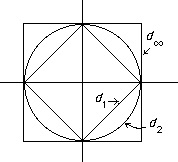
\includegraphics{images/geometryOfBalls.jpg}	
			\end{center}
	\end{enumerate}
\end{eg}

\begin{propo}
	Let $(X, d)$ be a metric space.
	\begin{enumerate}
		\item $X, \emptyset$ are both open and closed.
		\item If $\{U\}_{i \in I}$ is a family of open sets, then
			\begin{equation}
				\bigcup_{i \in I} U_i \quad \text{is open}
			\end{equation}
		\item If $\{U_1, ..., U_n\}$ is a finite family of open sets, then
			\begin{equation}
				\bigcap_{i = 1}^{n} U_i \quad \text{is open}
			\end{equation}
		\item If $\{F_i\}_{i \in I}$ is a family of closed sets, then
			\begin{equation}
				\bigcap_{i \in I} F_i \quad \text{is closed}
			\end{equation}
		\item Of $\{F_1, ..., F_n\}$ is a finite family of closed sets, then
			\begin{equation}
				\bigcup_{i = 1}^{n} F_i \quad \text{is closed}
			\end{equation}
			[Recall that singleton sets are closed, hence (5) implies that finite sets are closed]
	\end{enumerate}
\end{propo}

\begin{proof}
	\begin{enumerate}
		\item Let $x \in X$. Then $x \in B(x, 1) \subseteq X$, so $X$ is open. The test for openness of $\emptyset$ is vacuously true (i.e. there are no points to speak of: there are no $x \in \emptyset$ at all, hence for any such $x$, we have $x$ is ``contained'' in a ball in $\emptyset$).

			We have $\emptyset = X \setminus X, \; X = X \setminus \emptyset$ are closed.

		\item Let $x \in U = \bigcup_{i \in I} U_i$. Then there is some $i_0 \in I$ so $x \in U_{i_0}$, which is open, so there is an $\epsilon_x > 0$ such that
			\begin{equation}
				x \in B(x, \epsilon_x) \subseteq U_{i_0} \subseteq U
			\end{equation}

		\item Let $x \in V = \bigcap_{i = 1}^{n} U_i$. Then for each $i = 1, ..., n$, there is $\epsilon_i > 0$ so $B(x, \epsilon_i) \subseteq U_i$. Let $\epsilon = \min\{\epsilon_1, ..., \epsilon_n\} > 0$ and $B(x, \epsilon) \subseteq \bigcap_{i = 1}^{n} B(x, \epsilon_i) \subseteq V$
	\end{enumerate}

	For (4) and (5), use De Morgan's Laws and (2) \& (3) from above.
\end{proof}

\begin{defn}[Boundary]
	Given a metric space $(X, d)$, $A \subseteq X$, we define the boundary of A as
	\begin{equation}
		\partial A = \{x \in X : \forall \epsilon > 0 \; B(x, \epsilon) \cap A \neq \emptyset, \; \underbrace{B(x, \epsilon) \setminus A}_{B(x, \epsilon) \cap (X \setminus A)} \neq \emptyset \}
	\end{equation}
\end{defn}

\begin{remark}
	$\partial A = \partial(X \setminus A)$
\end{remark}

\begin{defn}[Interior]
	We let the interior of A
	\begin{equation}
		A^{\circ} = \bigcup \{U \subseteq X : U \subseteq A \land U \text{ is open} \}
	\end{equation}
\end{defn}

\begin{propo}[Characterizations of the Interior]
	If $(X, d)$, A are as above, then
	\begin{align}
		A^{\circ} &= \{x \in X : \exists \epsilon_x > 0 \; B(x, \epsilon_x) \subseteq A \} \\
			&= A \setminus \partial A \label{eq:A without its boundary}
	\end{align}
\end{propo}

\begin{proof}
	Let $x \in A$. Then we have either
	\begin{itemize}
		\item for some $\epsilon_x > 0, \; x \in \underbrace{B(x, \epsilon_x)}_{\text{open}} \subseteq A \implies x \in A^{\circ}$; or

		\item $\forall \epsilon > 0, \; B(x. \epsilon) \setminus A \neq \emptyset \implies \text{since } x \in A \cap B(x, \epsilon)$, we have $x \in \partial A$. Since $A^{\circ} \subseteq A$, we see that the the two equalities in \autoref{eq:A without its boundary} coincide.
	\end{itemize}
\end{proof}

\begin{defn}[Convergence]
	Let $(X, d)$ be a metric space, $(x_n)_{n = 1}^\infty \subseteq X$ and $x_0 \in X$. Then we say that $(x_n)_{n = 1}^\infty$ converges to the limit $x_0$, written
	\begin{equation}
		x_0 = \lim_{n \to \infty} x_n
	\end{equation}
	or
	\begin{equation}
		x_n \underset{n \to \infty}{\to} x_0
	\end{equation}
	if
	\begin{gather*}
		\forall \epsilon > 0 \; \exists n_\epsilon \in \bb{N} \\
		n \geq n_\epsilon \implies d(x_0, x_n) < \epsilon
	\end{gather*}
\end{defn}

\begin{remark}
	The limit, if it exists, is unique. Indeed, since
	\begin{gather*}
		x_0 = \lim_{n \to \infty} x_n \land y_0 = \lim_{n \to \infty} x_n
	\end{gather*}
	then
	\begin{gather*}
		\forall \epsilon > 0 \; \exists n_\epsilon, n_\epsilon' \in \bb{N} \\
		n \geq n_\epsilon \implies d(x_0, x_n) < \frac{\epsilon}{2} \\
		n \geq n_\epsilon' \implies d(y_0, x_n) < \frac{\epsilon}{2} 
	\end{gather*}
	But then if $n \geq \max\{n_\epsilon, n_\epsilon'\}$ we have
	\begin{equation*}
		d(x_0, y_0) \leq d(x_0, x_n) + d(x_n, y_0) < \epsilon
	\end{equation*}
	If this holds for all $\epsilon > 0, \; d(x_0, y_0) = 0$ so $x_0 = y_0$.
\end{remark}

\begin{eg}
	Let $(V, \Vert \cdot \Vert)$ be a normed vector space. A subset $\{e_n\}_{n = 1}^\infty \subseteq V$ is a \textbf{Schauder basis} provided that
	\begin{gather*}
		\forall x \in V \; \exists! \{x_n\}_{n = 1}^\infty \\
		x = \lim_{n \to \infty} \sum_{k=1}^{n} x_k e_k \quad \in V
	\end{gather*}

	Example: In $\ell_p \; (1 \leq p < \infty)$, let $e_n = (0, ..., 0, \underset{\text{n-th place}}{1}, 0, ..)$
\end{eg}

\begin{defn}[Accumulation points/Cluster Points and Isolated Points]
	We let $(X, d)$ is a metric space, $A \subseteq X$ as above, the set of accumulation points (or cluster points) be given
	\begin{equation}
		A' = \{x \in X : \forall \epsilon > 0 \; \left( B(x, \epsilon) \setminus \{x\} \right) \cap A \neq \emptyset \}
	\end{equation}
	(aka a punctured ball).

	Furthermore, we call elements of $A \setminus A'$ as isolated points.
\end{defn}

\begin{propo}
	Given $(X, d)$ as a metric space, $A \subseteq X$ as above, the set of all accumulation points
	\begin{equation*}
		A' = \{x \in X : x = \lim_{n \to \infty} x_n, \text{ where } (x_n)_{n = 1}^\infty \subseteq A \setminus \{x\} \}
	\end{equation*}
\end{propo}

\begin{proof}
	If $x \in A'$, let $x_1 \in \left( B(x, 1)\setminus\{x\} \right) \cap A$, and inductively let
	\begin{gather*}
		x_{n + 1} \in \left( B (x, \epsilon_n) \setminus \{x\} \right) \cap A
	\end{gather*}
	where $\epsilon+m = \min\{\frac{1}{n}, d(x, x_n)$.

	Then we have (exercise) that $x = \lim_{n \to \infty} x_n$, while $(x_n)_{n = 1}^\infty \subseteq A \setminus \{x\}$. [Notice the points $x_1, x_2, ..., x_n$ are distinct]

	The converse inclusion just uses the definition of limits. \qed
\end{proof}

\chapter{Lecture 11: Oct 2, 2017}\label{chp:lec11}

\section{Last time}

\begin{note}[3 Descriptions of interior $A^\circ$]
	\begin{equation*}
		\bigcup \{U \subseteq A : U \text{ open in } X\}, \{x \in X : \exists \epsilon_x > 0, \; B(x, \epsilon_x) \subseteq A \}
	\end{equation*}
\end{note}

\section{Continuing with Accumulation Points}\label{sect:accumulation points cont}

\begin{gather*}
	A' = \{x \in X : \forall \epsilon > 0, \left( B(x \epsilon) \setminus \{x \} \right) \cap A \neq \emptyset \} \\
	\text{Also } A' = \{x \in X : x = \lim_{n \to \infty} x_n, \; (x_n)_{n = 1}^\infty \subset A \setminus \{x \} \}
\end{gather*}

\begin{defn}[Closure]
	Given a metric space $(X, d)$ and $A \subseteq X$, define the closure of A by
	\begin{equation}
		\bar{A} = \cap \{F \subseteq X : A \subseteq F, \; F \text{ is closed in } X\}
	\end{equation}
	Of course, $A^\circ \subseteq A \subseteq \bar{A}$.
\end{defn}

\begin{thm}[Characterization of the Closure]
	Given a metric space $(X, d)$, $A \subseteq X$, the following sets are the same
	\begin{gather}
		\bar{A} \quad A \cup \partial A \quad A \cup A'
	\end{gather}
	(``meet'' set) $A_m = \{x \in X : \forall \epsilon > 0, \; B(x, \epsilon) \cap A \neq \emptyset \}$.

	(``limit'' set) $A_L = \{x \in X : x = \lim_{n \to \infty} x_n , \; \text{ where } (x_n)_{n = 1}^\infty \subseteq A \}$

	[The notations $A_L, A_m$ will not be used afterwards, we shall use $\bar{A}$.]
\end{thm}

\begin{proof}
	We have
	\begin{align*}
		\bar{A} &= \bigcap \{F \subseteq X : A \subseteq F, \; F \text{ closed}\} \\
			&= \bigcap \{X \setminus U : U \subseteq X \setminus A, \; U \text{ open in } X \}\\
			&= X \setminus \bigcup \{U : U \subseteq X \setminus A \; U \text{ open in } X \} \quad \text{De Morgon's Law} \\
			&= X \setminus [(X \setminus A)^\circ] \quad \text{(complement of interior)} \\
			&= X \setminus [(X \setminus A) \setminus \partial (X \setminus A)] \quad \text{(definition of $(X \setminus A)^\circ$)} \\
			&= X \setminus [(X \setminus A) \setminus \partial A] \\
			&= A \cup \partial A
	\end{align*}
	We thus have that $\bar{A} = A \cup \partial A$.

	Now if $x \in A \cup \partial A$, then $\forall \epsilon > 0, B(x, \epsilon) \cap A \neq \emptyset$ [i.e. either $x \in A \cap B(x, \epsilon)$, or $x \in \partial A$, so that $B(x, \epsilon) \cap A \neq \emptyset$]. Thus $A \cup \partial A \subseteq A_m$. Conversely, if $x \in A_m$, then, either
	\begin{itemize}
		\item $\exists \epsilon > 0, \; B(x, \epsilon) \subset A \implies x \in A^\circ \subseteq A$, or
		\item $\forall \epsilon > 0, \; B(x, \epsilon) \cap A \neq \emptyset$, in which case $x \in \partial A$.
	\end{itemize}
	Hence, $x \in A_m \implies x \in A \cup \partial A$ so $A_m \subseteq A \cup \partial A$.

	If $x \in A \cup A'$, then $\forall \epsilon > 0, \; B(x, \epsilon) \cap A \neq \emptyset$. Indeed, as above, either $x \in A$, so $\forall \epsilon > 0, x \in B(x, \epsilon) \cap A$, or $x \in A'$ so that $B(x, \epsilon) \cap A \supseteq (B(x, \epsilon) \setminus \{x\}) \cap A \neq \emptyset$. Hence $A \cup A' \subseteq A_m$.

	The definition of a limit of a sequence shows that $A_m = A_L$.

	Finally, consider
	\begin{align*}
		X \setminus (A \cup A') &\subseteq \{x \in X : \exists \epsilon_x > 0, \; B(x, \epsilon_x) \cap A = \emptyset (\implies B(x, \epsilon_x) \subseteq X \setminus A) \} \\
			&= (X \setminus A)^\circ \implies X \setminus [(X \setminus A)^\circ] \subseteq X \setminus [X \setminus (A \cup A')]
	\end{align*}
	Hence
	\begin{align*}
		\bar{A} = X \setminus [(X \setminus A)^\circ] &\subseteq X \setminus [X \setminus (A \cup A')] \\
			&= A \cup A'
	\end{align*}
	Hence $\bar{A} \subseteq A \cup A' \subseteq A_m = \bar{A}$, so $\bar{A} = A \cup A'$.\qed
\end{proof}

\begin{note}
	The ``limit'' set is going to help in A2
\end{note}

\section{Continuous Functions}\label{sect:cont functions}

\begin{defn}[Continuity]\label{defn:continuity}
	Let $(X, d_X)$ and $(Y, d_Y)$ be metric spaces. Let $f: X \to Y$ and $x_0 \in X$. We say that $f$ is continuous at $x_0$ if
	\begin{gather}
		\forall \epsilon > 0 \quad \delta > 0 \nonumber \\
		d_X(x, x_0) < \delta \implies d_Y(f(x), f(x_0)) < \epsilon \label{eq:continuous defn}
	\end{gather}
	We say that $f$ is continuous at the domain $X$ if it is continuous at each point in $X$.
\end{defn}

\begin{note}
	\begin{align*}
		\autoref{eq:continuous defn} &\iff f(B(x, \delta) \subseteq B(f(x), \epsilon) ) \\
			&\iff B(x, \delta) \subseteq f^{-1}B((f(x), \epsilon))
	\end{align*}
\end{note}

\begin{defn}[Neighbourhood]\label{defn:neighbourhood}
	In a metric space, a set $N$ is a \textbf{neighbourhood} of a point $x_0$, if $x_0 \in N^\circ$ (interior).
\end{defn}

\begin{thm}[Characterization of continuity at a point]\label{thm:char of cont at a point}
	If $(X, d_X), (Y, d_Y), f : X \to Y, x \in X$ are as above, then TFAE:
	\begin{enumerate}
		\item $f$ is continuous at $x_0$
		\item $\forall N$ of $f(x_0) \in (Y, d_Y)$, we have $f^{-1}(N)$ is a neighbourhood of $x_0$ in $(X, d_X)$.
		\item $x_0 = \lim_{n \to \infty} x_n \in (X, d_X) \implies f(x_0) = \lim_{n \to \infty} f(x_n) \in (Y, d_Y)$
	\end{enumerate}
\end{thm}

\begin{proof}
	$(1) \implies (2)$

	Given a neighbourhood $N$ of $f(x_0)$, $\exists \epsilon > 0, \; B(f(x_0), \epsilon) \subseteq N$. By assumption of $(1)$, $\exists \delta > 0, \; B(x_0, \delta) \subseteq f^{-1} (B(f(x_0), \epsilon) \subseteq f^{-1}(N)$. Thus $f^{-1}(N)$ is a neighbourhood of $x_0$.

	$(2) \implies (1) \implies (3)$

	Given $\epsilon > 0, \; B(f(x_0), \epsilon)$ is a neighbourhood of $f(x_0)$, so $f^{-1}(B(f(x_0), \epsilon))$ is a neighbourhood of $x_0$, and hence $\exists \delta > 0, \; B(x_0, \delta) \subseteq f^{-1}(B(f(x_0), \epsilon))$, which proves $(1)$.

	Now if $x_0 = \lim_{n \to \infty} x_n \in (X, d_X)$, then by definition, $\exists n_\delta \in \bb{N}$ such that if $n \geq n_\delta, \; x_n \in B(x_0, \delta)$. But then for $n \geq n_\delta$, we have
	\begin{equation*}
		f(x_n) \in f(B(x, \delta)) \subseteq B(f(x_0), \epsilon)
	\end{equation*}
	and hence $f(x_0) = \lim_{n \to \infty} f(x_n)$.

	$(3) \implies (1)$ which we shall prove by contrapositive, i.e. $\neg (1) \implies \neg (3)$

	If $\neg (1)$, then $\exists \epsilon > 0, \; \forall \delta > 0$
	\begin{equation*}
		B(x_0, \delta) \not\subset f^{-1}(B(f(x_0), \epsilon)).
	\end{equation*}

	Hence for each $n \in \bb{N}$, we may find
	\begin{equation*}
	 	x_n \in B(x_0, \frac{1}{n}) \setminus f^{-1}(B(f(x_0), \epsilon)
	\end{equation*}
	Given  $\epsilon' > 0, \; \exists n_{\epsilon'} \in \bb{N}, \; \forall n_{\epsilon'} \geq \frac{1}{\epsilon'}$. Then for $n \geq n_{\epsilon'}, \; x_n \in B(x_0, {\epsilon'})$ thus $\lim_{n \to \infty} x_n = x_0$. However, each $f(x_n) \notin B(f(x_0), \epsilon)$, so $f(x_n) \underset{n \to \infty}{\not\to} f(x_0)$.

\end{proof}

\end{document}
% Document End